\begin{savequote}[8cm]
  ``I just wondered how things were put together.''
  \qauthor{Claude Shannon}
\end{savequote}
\makeatletter
\chapter{Experiments}

\section{Experiments}

\section{Test Data}

Test Data was generated based on the testing requirements for this research. In order to robustly test the different pose-estimation procedures / 3D-registration methods we generated data from a variety of scenes. These scenes include both in-door and out-door scenes, scenes with large amounts of texture and scenes with little to no texture. We also captured scenes which may cause confusion for algorithms which rely on texture information. This data typically has many items which look similar locally but are actually different objects within the scene globally. \\

Moreover, our test-data also measure's each algorithm's ability to register different camera movements by localizing them to different scenes. Different camera motions captured include: camera translation and zooming as well as different axes of rotation. \\

Some frames from the original test-set are shown in appendix \ref{AppendixA}. The first scene: the Apartment Texture Rotate scene was taken by rotating the camera around the y-axis across an apartment. This scene contains plenty of textural information. The Apartment Texture X Axis scene is similar in terms of texture but contains both x and y axis rotation. This tests the Volume Phase Registration algorithm's ability to handle multiple axes of rotation. \\

The boxes scene was captured under arbitrary-rotation, translation and zoom-in/out camera motions. It contains some useful information on the boxes themselves, however the texture on the carpet is of little to no use for most feature based registration methods. The Desk Texture Translation scene contains a desk with a desktop computer and several items on it. The In-door space with texture-confusion contains a set of chairs and picture frames which look similar to eachother locally but may cause confusion for registration techniques which rely on local features.  \\

The kitchen scene was captured with both translation and zoom camera movements. The scene contains very little texture and the color is predominantly white. The Office textured blind-spot rotation scene is a textured office scene where the camera is rotated about the y-axis. The scene is focused on a large divider which seperates two desks. The divider may confuse registration methods which rely too heavily on minimization by aligning the large divider in priority rather than taking into acount the smaller details of the scene. \\

The Office scenes contain a decent amount of usable texture and different sets were created by translating, rotating about the y-axis and rotating about the x-axis. Other office scenes, where the camera has objects in both the foreground and the background and where the camera is lifted and rotated whilst focusing on an office desk/chair. \\

Some out-door scenes were also captured around the university. Scenes are captured with both rotation and translation camera movements. These scenes are also labelled as being susceptable to texture confusion.

\section{Analysis Tools}

In order to test different registration methods. Algorithms were written in C/C++ using both Visual Studio (2012 and 2015) on a Windows (7 \& 10) machine and code-blocks 16 on an Ubuntu machine. All source code is made available online at: https://github.com/lukes611/phdThesis. In order to measure registration algorithms we use the error metrics described in the ERROR METRICS SECTION section.  

\section{Algorithms}

Different 3D-registration algorithms were implemented to test the Fourier Volume Registration (FVR) method. We compared with Feature Matching methods because these methods are still dominant and very successful in image processing and computer vision. In this research we aimed to show that FVR was competitive with these feature matching methods whilst beating them in certain contexts (such as little textuere or scenes where texture confusion may occur). \\ 

We test with both 2D feature matching, where the features are found and matched between a pair of 2D-images, then RANSAC is used with the corresponding matches and true 3D point to compute pose. The pose is then used to reconstruct the scene. We found that SURF performed best out of the other feature matching methods, so we use SURF in our 2D feature matching algorithm. The 2D feature matching method is limited as it cannot register frames which have too few features or frames which contain texture confusion. It is also not able to handle wider base-lines. \\

We also test 3D-feature matching using an implementation of SIFT in 3D. This algorithm was tested and written in C/C++ and is also susceptable to failed registration in scenes with too few features and texture confusion but it shouble be more able to handle wider base-lines than the 2D counterpart as it works in 3D. //

Another algorithm we test against is ICP or Iterative Closest Point. This method has become very popular in 3D reconstruction and works well on most scene types. One disadvantage is that this method may get stuck in a minima and fail to register, this can occur especially when registering wider baselines. \\

The other method we test with is PCA or Principal Components Analysis is actually used to find the mean and principal components of a multi-dimensional data-set. This is useful for registration purposes as it works on wide-baselines, is very fast and provides additional information about a scene. The downside is that is is very susceptable to noisey or mis-aligned data. Our FVR method actually makes use of information from PCA so it is good to compare the two to find out what improvements if any are made by FVR. \\

The final algorithm tested is the proposed FVR algorithm, which uses both PCA and Fourier Phase Correlation to find the registration transformation between two 3D data-sets. This algorithm was proposed to handle general transformations about any rotation axis, translation axis as well as handle scaling. It was also designed to be able to handle noisey data, data with texture-confusion and data with little to no texture making it a viable option in the 3D registration and pose estimation research areas.


\section{Qualitative Experiments}

Our Qualitative experiments were performed by using different algorithms to generate 3D reconstructed scenes. 

\section{Quantitative Experiments}

\subsection{Camera Movement Experiments}

\subsection{Pose Estimation Experiments}

\subsection{Noise Experiments}




\begin{figure*}[t] 
        \centering
        \begin{subfigure}[b]{2.0in}
                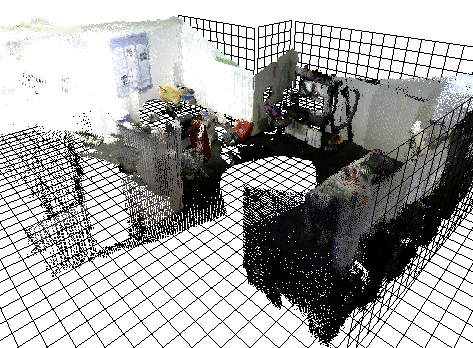
\includegraphics[width=2.0in]{images/ch2/unit21}
                \caption{Apartment}
                \label{fig:RECON_UNIT}
        \end{subfigure}%
        \begin{subfigure}[b]{2.0in}
                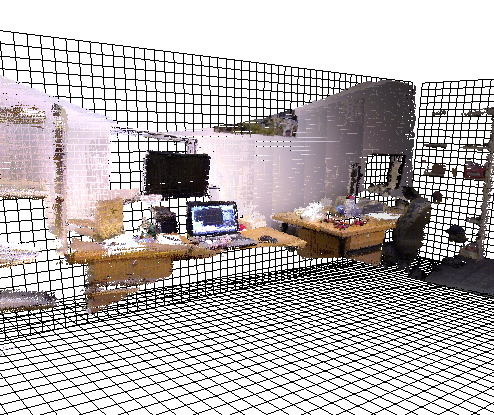
\includegraphics[width=2.0in]{images/ch2/officeA}
                \caption{Office}
                \label{fig:RECON_OFFICE}
        \end{subfigure}%
        \begin{subfigure}[b]{2.0in}
                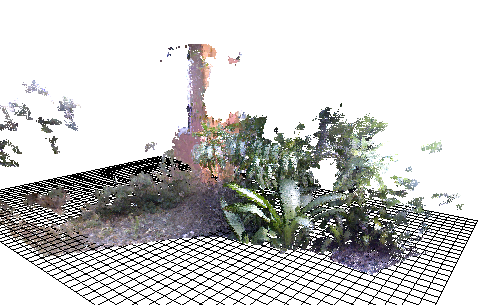
\includegraphics[width=2.0in]{images/ch2/outdoorA}
                \caption{Garden}
                \label{fig:RECON_GARDEN}
        \end{subfigure}
       \caption{Reconstructed Scenes.}
       \label{fig:RECONSTRUCTIONS}
\end{figure*}


\subsection{Codec Evaluation \& Comparison Techniques}

Codec evaluation involves comparing storage requirements between the original model and codec output. In the case of lossy codecs, a quantitative quality metric is also required. Compression metrics are easy to compute, quality metrics are more involved and there have been many proposed techniques. Quality metrics compare the distortion created by the codec relative to the original model. Two measurements are usually performed, the distance from the compressed model to the original and the distance from the original to the compressed model. Quality metrics are split into empirical and perceptual based metrics. Empirical metrics measure geometric error and perceptual metrics estimate human perception. Perception based metrics are a part of psychophysics research. For a more in-depth survey of these methods, see work by Bubill \textit{et al.} \cite{Bulbul11Assessing}.

\subsubsection{Compression Metrics}

In the context of 3D model compression, the file size of both, the compressed model and the original are compared. Alternatively, the file size of the compressed model from one codec can be compared to the file size of the same model compressed using another codec. The compression ratio ($CR$), defined as the original file size divided by the compressed file size, is a measure of compression performance. Another metric used is called the bit rate, different bit rates are used depending on the representation being compressed. The mesh representation uses bits per vertex (bpv) and bits per triangle (bpt), the volumetric representation uses bits per voxel and the point cloud representation uses bits per point.

\subsubsection{Empirical Error Metrics}

The following metrics are used to assess the error between two data samples. For two points, $p$ \& $q$, in $\Re^3$ space, the basic euclidean distance metric,
$$
ED(q,p) = \sqrt{(q_x - p_x)^2 + (q_y - p_y)^2 + (q_z - p_z)^2}
$$,
the absolute error,
$$
AE(q,p) = \|q_x - p_x\| + \|q_y - p_y\| + \|q_z - p_z\|
$$
and the squared error $SE$, 
$$
SE(q,p) = (q_x - p_x)^2 + (q_y - p_y)^2 + (q_z - p_z)^2
$$
are often used as a basis for other metrics. 3D models can be sampled into a set of points in $\Re^3$. Using these samples, the following metrics can be used: sum of distances ($SOD$), sum of absolute differences ($SAD$), sum of squared errors ($SSE$), mean square error ($MSE$) and root mean square error ($RMS$). Since the two models may be sampled differently, the minimum error from one sample to the others is used. These metrics are defined below using two point sets, $A$ \& $B$ where the length of these sets is $M$ and $N$ respectively.
$$
SOD(A,B) = \sum_{k=0}^{M} \min_{b \in B}(ED(A_k,b))
$$

$$
SAD(A,B) = \sum_{k=0}^{M} \min_{b \in B}(AE(A_k,b))
$$

$$
SSE(A,B) = \sum_{k=0}^{M} \min_{b \in B}(SE(A_k,b))
$$

$$
MSE(A,B) = \frac{1}{M}SSE(A,B)
$$

$$
RMS(A,B) = \sqrt{MSE(A,B)}
$$

For each of these metrics, $METRIC(A,B) \neq METRIC(B,A)$. Therefore, these methods are often averaged (below). This is termed the average metric (AM), as opposed to the minimum metric (MM) which is the smallest value of the two.

$$
AvgError = \frac{Metric(A,B)+Metric(B,A)}{2}
$$

Another metric, the Hausdorff distance ($HD$) is a measure of overall shape similarity. It is defined as the largest value of the maximum distances between objects from $A$ to $B$ and from $B$ to $A$. For example, for two objects $A$ \& $B$, the Hausforff distance $HD$, from $A$ to $B$, is defined as,
$$
HD(A,B) = \max(D(A,B),D(B,A))
$$
where $D(A,B)$ is defined as,
$$
D(A,B) = \{a \in A \| \max(dist(a,B)\}
$$
and $dist(a,B)$ is defined below.
$$
dist(a,B) = \{b \in B \left| \min(\|a-b\|)\right.\}
$$

\subsubsection{Human Perception Based Metrics}

Lavoue \textit{et al.} \cite{Lavoue06Perceptually} devised a metric based on structural distortion, this method correlates well with human perception. It is based on the SSIM method of Wang \textit{et al.} \cite{Wang04Image}, which is a popular image metric. Lavoue \textit{et al.} call their method the, Mesh Structural Distortion Measure (MSDM). An updated version of this metric was also developed \cite{Lavoue11Multiscale}.

\paragraph{Laplacian Metric}

Karni \& Gotsman \cite{Karni00Spectral} developed their own on-line metric for use during their spectral based codec. It is based on the laplacian and measures the difference between two objects in terms of their smoothness. 

\paragraph{Elastic Deformation Based Metric}

Bian \textit{et al.} \cite{Bian09Evaluation} developed a novel metric, useful for both on and off-line model comparison. The algorithm is based on the theory of strain fields. A strain field is a metric derived from elasticity, it is used to describe the deformation of some object which has elastic properties. Using this concept, both models are treated as having elastic properties in order to perform quality assessment.

\paragraph{Saliency Based Metrics}

Howlett \textit{et al.} \cite{Howlett04Experimental} and Lee \textit{et al.} \cite{Lee05Mesh} both presented work aimed at determining salient features in 3D models. They incorporated these findings in their own metrics. Howlett \textit{et al.} used a human gaze detection device to study the psychophysical effects of viewing 3D objects. Both of these metrics are based on preserving the sections of the object in which any distortion would be visibly noticeable to humans.

\paragraph{The Depth Difference Metric}

Krivokuca \textit{et al.} \cite{Krivokuca12New} developed a perceptual based metric for the off-line quality assessment of 3D models. This method is independent of model representation and is based on generating multiple depth maps from different orthographic perspectives. It improves upon both the Hausdorff distance and RMS error and is good at detecting both small and large geometric errors. Krivokuca \textit{et al.} call their method, the Depth Difference (DD). It works by comparing orthographic depth maps from both the original and compressed models. First a difference depth image is calculated ($DDI$) from orthographic depth maps of the original object ($DIO$) and of the compressed object ($DIC$). The $DDI$ is calculated using element-wise matrix subtraction,

$$
DDI = DIO - DIC
$$

Then the average depth distance value ($ADD$) is calculated from the $DDI$ matrix, this equation is presented below.

$$
ADD = \frac{1}{MN} \sum_{y=0}^{M} \sum_{x=0}^{N} DDI_{y,x}
$$

This $ADD$ value is then summed up and averaged over different orthographic views, this average is the Depth Difference.

